% The paper's skeleton: one file per section, figures and tables from paper/figs/out/ (generated; do not edit there).
% Every result sentence carries a trailing comment naming its FINDINGS section (s##) and its paper/CLAIMS.md row;
% paper/tex/check_tex.py checks the numbers against those files.
\documentclass[11pt]{article}
\usepackage[utf8]{inputenc}
\usepackage[T1]{fontenc}
\usepackage[margin=1in]{geometry}
\usepackage{amsmath}
\usepackage{booktabs}
\usepackage{graphicx}
\usepackage[numbers,sort&compress]{natbib}
\usepackage{xcolor}
\usepackage[hidelinks]{hyperref}

\graphicspath{{../figs/out/}}
\newcommand{\code}[1]{\texttt{#1}}
\newcommand{\TODO}[1]{\textcolor{red}{[TODO: #1]}}

\title{\TODO{title}}
\author{\TODO{authors}}
\date{}

\begin{document}
\maketitle

\begin{abstract}
\TODO{abstract, written last}
\end{abstract}

% Section 1: stub (audit outline item 1).
\section{Introduction}
\label{sec:intro}

\TODO{Introduction: the question (does a matrix-weighted colour VQ beat C3DGS's own at equal rate, and does the lead survive fine-tuning), the pre-registered design, the contributions. Written after Sections 4 and 5.2.}

% Related work. Literature, not results: citations only from references.bib (verified 2026-10-23); a needed reference
% that is not in it is a \TODO{cite: ...} marker, not an entry. OGC's and Do et al.'s content from kaggle/RELATED_WORK_OGC.md
% (literature notes, paraphrased). A sentence that uses this project's results cites its CLAIMS row, as elsewhere.
\section{Related work}
\label{sec:related}

\paragraph{Compressing 3D Gaussian Splatting.}
3D Gaussian Splatting represents a scene by millions of anisotropic Gaussians, each with a position, a covariance, an opacity and a view-dependent colour stored as spherical-harmonic (SH) coefficients, which make up most of each Gaussian's stored floats \citep{kerbl2023gaussian}.
Compression methods for it divide into those that learn a compact representation during training and those that start from a trained model \TODO{cite: a survey of 3DGS compression, e.g. Bagdasarian et al., 3DGS.zip}.
Training-time methods prune Gaussians with learned masks, learn colour codebooks or hash-grid colour fields jointly with the scene, or anchor Gaussians to structured features \TODO{cite: Lee et al. 2024 (Compact 3D Gaussian representation); Navaneet et al. 2024 (CompGS); Girish et al. 2024 (EAGLES); Lu et al. 2024 (Scaffold-GS); Chen et al. 2024 (HAC)}.
Post-training methods prune Gaussians, reduce the SH degree, or vector-quantise (VQ) the parameters of a trained model, usually followed by a short fine-tuning \TODO{cite: Fan et al. 2024 (LightGaussian); Papantonakis et al. 2024 (reducing the memory footprint of 3DGS)}.
This paper works in the post-training setting, and its host is C3DGS \citep{niedermayr2024compressed}.

C3DGS scores each colour and shape parameter by its sensitivity, the magnitude of the gradient of the rendered training images' total energy (the sum of their pixel values) with respect to it, accumulated over the training views, and gives each Gaussian the largest sensitivity among its colour parameters and, separately, among its shape parameters \citep{niedermayr2024compressed}. % C3DGS paper Sec. 4.1, Eq. 3, App. E; code at 2a234af5: compress.py:40-84, 154-156
It removes the Gaussians whose colour sensitivity is zero, clusters the colours of the others into a codebook with sensitivity-weighted $k$-means, and lets the Gaussians whose colour sensitivity lies above a threshold keep their own colour \citep{niedermayr2024compressed}. % Sec. 4.1, Eqs. 5-6, App. E; compression/vq.py:37-60, 78-117, 155, 250-253; arguments/__init__.py:75, 92
It clusters the shape in the same way, as normalised covariance matrices with a separate scale factor per Gaussian, quantises every parameter except the position to 8 bits and stores positions as 16-bit floats, fine-tunes the model with the quantisation in the loop, and stores the arrays, sorted in Morton order, with DEFLATE compression \citep{niedermayr2024compressed}. % Sec. 4.1, App. F, Sec. 4.2, Sec. 4.3; compression/vq.py:194-238; scene/gaussian_model.py:78-88, 182-198, 450-451, 463, 575; compress.py:231; arguments/__init__.py:72, 90; finetune.py:12-24
This paper changes only C3DGS's colour codebook and keeps the rest of its pipeline as released, fine-tuning included (Section~\ref{sec:setup}). % Am17 b

\paragraph{Observation-Gram compaction.}
OGC \citep{pietroszek2026only} weights a Gaussian's SH colour by what the training cameras saw.
For each Gaussian it accumulates a $16\times16$ observation Gram matrix over the SH basis: a sum over the training views of the outer product of the SH basis at the viewing direction, weighted by the Gaussian's compositing weights in that view, so that a colour error in a direction no training camera observed costs nothing \citep{pietroszek2026only}.
In its own pipeline OGC uses the matrix to project the colour onto fewer SH degrees, to allocate coefficients among Gaussians, and as the metric of a generalised Lloyd VQ of the AC coefficients \citep{pietroszek2026only}.
Hosted in C3DGS, it replaces only C3DGS's colour VQ with that Gram-metric Lloyd VQ on all 16 SH rows, keeps C3DGS's pruning, shape VQ, fine-tuning and container, and reports a paired PSNR gain over its reproduction of C3DGS of +0.49 dB before C3DGS's fine-tuning and +0.09 dB after it, on nine Mip-NeRF 360 scenes \citep{pietroszek2026only,barron2022mipnerf360}. % OGC's Table 1, as A4 and A5 state it; A4, A5
Its paper states a ridge of $10^{-6}$ in the VQ's codeword update, while its released code defaults to $10^{-3}$; this paper uses the code's value (Section~\ref{sec:setup}). % RELATED_WORK_OGC.md 2 b; Am17 b; B7; CLAIMS Gap 12
This paper replicates OGC's host comparison under a pre-registered protocol (Section~\ref{sec:replication}), tests whether the lead survives fine-tuning at equal rate (Section~\ref{sec:finetuning}), and dissects which parts of OGC's VQ carry the lead (Section~\ref{sec:dissection}). % Am17; Am19

Do, Chou and Cheung \citep{do2026transforming} also weight SH coefficients by how they are observed, but with one global Gram matrix over all basis functions of all splats, approximated as a product of spatial, directional and colour factors.
Its square root orthonormalises the coefficients before uniform scalar quantisation and entropy coding; the method codes sparse voxel splats rather than 3DGS models, and has no VQ \citep{do2026transforming}.

\paragraph{Second-order and observation-weighted quantisation.}
Weighting a quantiser's error by a second-order model of the loss predates both methods.
In neural-network compression the Hessian of the loss, or its Gauss--Newton approximation, has been used to choose which weights to prune \TODO{cite: LeCun et al. 1990 (Optimal Brain Damage); Hassibi and Stork 1993 (Optimal Brain Surgeon)}, to weight the $k$-means clustering of weights \TODO{cite: Choi et al. 2017 (Towards the limit of network quantization)}, to set per-layer bit widths \TODO{cite: Dong et al. 2019 (HAWQ)}, and to quantise weights one at a time while the remaining weights compensate \TODO{cite: Frantar and Alistarh 2022 (OBQ); Frantar et al. 2023 (GPTQ)}.
Layer-wise quantisers that minimise the error of a layer's outputs on calibration data weight the error by the Gram matrix of the layer's inputs, which is the same construction applied to activations \TODO{cite: Nagel et al. 2020 (AdaRound); Frantar et al. 2023 (GPTQ)}.
For one Gaussian the rendered colour is linear in its SH coefficients, ignoring the clamp of negative colours, so a Gauss--Newton metric of the image error with respect to those coefficients has the form of OGC's observation Gram; the metric used in this paper is a 16-probe estimate of it, equal to OGC's Gram in expectation by construction (Section~\ref{sec:setup}). % Am17 b; A12; RELATED_WORK_OGC.md 2 a, 3
C3DGS's sensitivity is a first-order, scalar counterpart: one weight per Gaussian, the largest gradient magnitude among its colour parameters, so its clustering distance does not distinguish viewing directions. % C3DGS paper Sec. 4.1, Eq. 5; compress.py:154; compression/vq.py:37-60
OGC's scalar variant, the trace of the Gram matrix times the identity, lies between the two, and Section~\ref{sec:gram-trace} tests the full matrix against it. % Am17 b; B1
This project began with a Gauss--Newton-weighted VQ of the SH codebook in gsplat's PNG codec (GN-VQ), which was never compared with OGC on a gate scene and was retired before the replication (Section~\ref{sec:gnvq}). % s17; Am17 a; C5, D6

% Section 2: setup and protocol. Facts only, each sourced: FINDINGS sections as s##, paper/CLAIMS.md rows by ID,
% kaggle/PREREG_GN.md amendments as Am## (e.g. Am17 b). One sentence per line; check_tex.py reads the trailing comments.
\section{Setup and protocol}
\label{sec:setup}

\subsection{Host, checkpoints and code}

All experiments ran inside the C3DGS compression pipeline \citep{niedermayr2024compressed} at commit \code{2a234af5}, on INRIA's published 30k checkpoints of 3D Gaussian Splatting \citep{kerbl2023gaussian}. % Am13 b; Am15 d; A1 (the common limits block)
C3DGS's source was not edited; the build and run deviations were recorded: a \code{<cstdint>} rebuild of one extension, a wrapper that chunks \code{torch.linalg.eigh} and \code{det} (8,192 matrices per call) after the unchunked call failed in cuSOLVER, and a fix that lets C3DGS's own evaluation run when the training images are kept on the CPU. % s14, s17, s18, s19; E1, E7
On the development scene train, the host reproduced C3DGS's published row within 0.020 dB in PSNR and 0.134\% in size. % s14; E3
OGC's colour VQ \citep{pietroszek2026only} was run from its released code at commit \code{49ccae72} \citep{pietroszek2026ogccode}, unedited, under that code's public licence, the PolyForm Noncommercial License 1.0.0, which permits noncommercial research use; none of its files is in this project's repository or result bundles. % the repository's LICENSE at 49ccae72 (public); Am18 c; E12 (its licence statement only)
All runs used two NVIDIA T4 GPUs on Kaggle and one software image per experiment. % s19, s21; A1 (the common limits block)

\subsection{Scenes}

The gate scenes were INRIA's checkpoints of seven scenes: bonsai, counter, kitchen and room from Mip-NeRF 360 \citep{barron2022mipnerf360}, truck from Tanks and Temples \citep{knapitsch2017tanks}, and drjohnson and playroom from Deep Blending \citep{hedman2018deep}. % Am15 d; Am17 d; A1 (the common limits block)
INRIA's checkpoints of these scenes were chosen as the gate before this project had fetched, loaded or rendered any of them, and before E5's code no splat value, render or metric from them had been read beyond camera counts, image sizes and splat counts, under a header-read rule written in advance. % Am15 d ("has not fetched, loaded or rendered"); Am15 note i; Am17 a
Three INRIA scenes, train, treehill and flowers, served as development scenes and are never gate scenes. % Am16 b; Am19 b; CLAIMS group G limits
\emph{Disclosure.} Earlier experiments of this project used bonsai, counter, kitchen, room and truck with its own gsplat checkpoints, and OGC's paper reports bonsai, counter, kitchen and room in its C3DGS host. % Am15 d (kept by Am17 d); A1 (the disclosure in its limits column)
The fine-tuning test of Section~\ref{sec:finetuning} reuses the same seven scenes, and its hypothesis was formed after the replication's results on them, so it is a pre-registered test on these scenes and not a held-out claim. % Am19 c; CLAIMS group F limits

\subsection{Rows and the forked process}

Each process runs C3DGS once and forks it at the colour VQ: C3DGS's own VQ (\code{c3dgs}) runs first, unchanged, and the other rows are computed at the same call from the same inputs, while the geometry VQ runs once and is shared. % Am17 b; Am15 b
The model, the quantizers and the random states are copied when C3DGS's compression returns, each row's colour table is installed into a restore of that copy, and every row is saved before any row is evaluated. % Am17 b; Am15 b
The rows are C3DGS's VQ and OGC's \code{gram\_kmeans} under its three metrics: the identity (\code{ogc\_plain}), the trace weight $\operatorname{tr}(G_i)/16\cdot I$ (\code{ogc\_scalar}) and the per-splat $16\times16$ Gram matrix $G_i$ (\code{ogc\_gram}, OGC's method). % Am17 b
OGC's call is the same in every row except for the metric: $K$~=~4,096, 15 iterations, seed 0, a chunk of 25,000 splats and its code's default ridge $\lambda = 10^{-3}$, with its own initialisation, reseeding and final assignment. % Am17 b
$\lambda = 10^{-3}$ is also the value that held-out-view cross-validation chose on both development scenes where it was run. % s17; B7
The metric $G$ is this project's per-splat Gauss--Newton metric over all training views, a 16-probe estimate equal in expectation to OGC's observation Gram by construction; on train its total trace measured 0.919 of the exact Gram's, a shortfall the files do not explain. % Am17 b; s16; E4, A12 ("the trace shortfall's cause is not settled"); RELATED_WORK_OGC.md section 3
A derived reimplementation of OGC's VQ (\code{ogc\_gram\_ours}) ran beside OGC's in every process, report only. % Am18 d; A6
Fine-tuning, where a test calls for it, is C3DGS's own 5,000-iteration fine-tuning, started from the copy with the row's table installed; the labels were checked to survive it. % Am17 b; Am19 c

\subsection{Rate and the BD measures}

The rate knob is C3DGS's colour threshold, $6\times10^{-7}\cdot 3^{j}$ at $j = -1, 0, +1$, with $K$ fixed: on train the threshold spanned 2.49 times in bytes and $K$ only 1.02 times. % Am17 d; s15; E10
Each point is one process with seed 0, and $j = 0$ also has a second process with seed 1. % Am17 d; Am19 c
A row's curve is its test PSNR against $\log_{10}$ of its compressed \code{.npz} bytes at the three points, fitted by the parabola through them. % s19 "How the numbers are computed"
BD-PSNR averages the difference of two parabolas over the range of $\log_{10}$ bytes the two curves share, and is defined whenever the byte ranges overlap. % s19 "How the numbers are computed"
BD-rate fits $\log_{10}$ bytes against PSNR and averages over the shared PSNR range; it is undefined without one and is not interpreted when that range is below 0.1 dB. % s19; s21 secondary 2; F3

\subsection{Evaluation}

The primary evaluation is protocol~ii: INRIA's evaluation set-up, with the dataset's own test images at the checkpoint's training resolution and renders quantised to 8 bits, scored by this project's PSNR, SSIM and LPIPS-VGG modules. % Am12 a; s13
Every row was also evaluated by C3DGS's own evaluation, which scores float renders with its own SSIM and LPIPS code. % Am17 b, e.2; s14
The two protocols disagree by a scene-dependent amount: C3DGS's evaluation reads higher by 0.429 dB on kitchen and 0.167 dB on bonsai, and by 0.007 to 0.035 dB on the other five, for reasons the files do not show. % s20; E14

\subsection{Pre-registration history}

Every experiment was pre-registered in a dated amendment committed before its code or data, and no rule was edited after results existed; later changes are new dated amendments or notes. % PREREG_GN.md (every amendment's heading)
The project began with a Gauss--Newton-weighted VQ (GN-VQ) inside gsplat's PNG codec; its first gate failed on the size rule, and the project continued after that result as a declared deviation. % s9; D1; Am7 b
A gate of GN-VQ inside C3DGS was registered with a pilot on train, and was withdrawn before any gate-scene data once the pilot showed its primaries were about zero or compared unequal codebooks. % Am15; Am16 a; s16; D5
An exploratory dissection on the development scenes then found that OGC needed 14.42\% fewer bytes than GN-VQ at equal quality on train, and GN-VQ was retired from any gate. % s17; Am17 a; D6
The replication of OGC inside C3DGS (E5, Section~\ref{sec:replication}) and its pilot on train were registered next, with OGC's source chain and the derived reimplementation in the following amendment. % Am17; Am18
The fine-tuning curves (E6, Section~\ref{sec:finetuning}) were registered after E5's verdict, and the dissection of the fine-tuning result (E7) after E6's. % Am19; Am20

\subsection{Criteria, noise and the standard error}

Each primary $P$ is one BD-PSNR per scene, and the registered verdict has three criteria: $\bar P > 0$, $P > 0$ on at least $\lfloor (7n+9)/10 \rfloor$ scenes (5 needed when $n = 7$), and $\bar P > 2\,\mathrm{SE}_{\mathrm{noise}}$, every compared value rounded to 9 decimals, with the verdict order incomplete, then fail, then pass. % Am17 d; Am17 Note2C2, Note2C7 (amendment items, not CLAIMS rows); Am19 c
$\mathrm{SE}_{\mathrm{noise}}$ is seed noise only: the two $j = 0$ seeds' paired difference, pooled over the scenes as $\mathrm{SD}_{\mathrm{pool}}$ with one degree of freedom per scene, and divided by $\sqrt{2n}$; it does not include how $P$ varies from scene to scene. % s19 "How the numbers are computed"; s21
A later re-reading found that $\mathrm{SD}_{\mathrm{pool}}/\sqrt{n}$ is the standard error that matches a mean of one seed-0 curve per scene, larger than the registered one by $\sqrt{2}$. % s25; A1
Under it every criterion of E5 and E6 still holds, and the registered verdicts stand under their pre-registered rule; Sections~\ref{sec:replication} and~\ref{sec:finetuning} report both. % s25; A1, F1

% Section 3: the replication (E5, H1). Sources: FINDINGS s19-s21, s25; CLAIMS A1-A6, A9, A10, F2, G8.
% One sentence per line; each result sentence names its FINDINGS section (s##) and CLAIMS row in its trailing comment.
\section{Replication}
\label{sec:replication}

\subsection{Hypothesis and test}

The replication (E5) asked whether, inside C3DGS and at equal rate over the three colour thresholds, OGC's Gram-metric VQ beats C3DGS's own colour VQ (P1, BD-PSNR of \code{ogc\_gram} against \code{c3dgs}) and beats the same Lloyd with the metric's trace (P2, \code{ogc\_gram} against \code{ogc\_scalar}), on the seven gate scenes. % Am17 d
It runs OGC's released VQ code (\code{gram\_kmeans}, unedited) on this project's estimate of OGC's metric (Section~\ref{sec:setup}), not on OGC's own Gram computation. % Am17 b; s16; E4
Both primaries were tested with the three criteria of Section~\ref{sec:setup}, before fine-tuning, on four processes per scene. % Am17 d; s19

\subsection{Result (pre-registered)}

E5 passed as pre-registered: both primaries met all three criteria with $n = 7$, no scene dropped, no primary row or value missing, and no process deferred, cut, rerun or stopped. % s19 "The verdict"; A1
OGC's VQ led C3DGS's own on every scene, with $\bar P_1 = 0.3558$ dB against $2\,\mathrm{SE}_{\mathrm{noise}} = 0.0065$ dB, from 0.1486 dB on truck to 0.4841 dB on bonsai (Table~\ref{tab:t1}). % s19 per-scene table; A2
The Gram metric led its trace on every scene, with $\bar P_2 = 0.1874$ dB against $2\,\mathrm{SE}_{\mathrm{noise}} = 0.0003$ dB. % s19 per-scene table; B1
Every one of the 14 per-scene values lay more than $2\,\mathrm{SE}_{\mathrm{noise}}$ above zero. % s19 "The verdict"; A1

\begin{table}[t]
\centering
\small
\caption{E5's primaries per scene (dB), as the verdict compared them (9 decimals). $D_s$ is the mean of the two $j = 0$ processes' paired difference. Pre-registered; generated from the committed bundles.}
\label{tab:t1}
% FINDINGS section 19, The verdict (E5, kaggle/gn_e5/S1-S3/gn5/)
% generated by paper/figs/t1_e5_primaries.py from committed bundles; do not edit
\begin{tabular}{lrrrr}
\toprule
Scene & P1 (dB) & P1 pair, $D_s$ & P2 (dB) & P2 pair, $D_s$ \\
\midrule
bonsai & 0.484060073 & 0.662099426 & 0.320522033 & 0.418902629 \\
counter & 0.319226727 & 0.449111462 & 0.165453427 & 0.205868244 \\
kitchen & 0.411145219 & 0.631160777 & 0.275679656 & 0.378012426 \\
room & 0.386923539 & 0.540365366 & 0.175005021 & 0.218052008 \\
truck & 0.148587944 & 0.248380899 & 0.100030562 & 0.149408519 \\
drjohnson & 0.276526313 & 0.446854649 & 0.128071281 & 0.170944156 \\
playroom & 0.464370802 & 0.689506991 & 0.147096105 & 0.180252437 \\
\midrule
$\bar P$ ($n = 7$) & 0.355834374 &  & 0.187408298 &  \\
SD\_pool & 0.012122221 &  & 0.000627531 &  \\
SE\_noise = SD\_pool / $\sqrt{14}$ & 0.003239800 &  & 0.000167715 &  \\
2 $\times$ SE\_noise & 0.006479600 &  & 0.000335429 &  \\
scenes with P > 0 & 7 (5 needed) &  & 7 (5 needed) &  \\
\bottomrule
\end{tabular}

\end{table}

Across the seven scenes P1 had a standard deviation of 0.1175 dB ($t = 8.01$) and P2 one of 0.0805 dB ($t = 6.16$); these scene-level statistics were not pre-registered. % s19 "Exploratory"; A3
Under the standard error that matches one curve per scene, $\mathrm{SD}_{\mathrm{pool}}/\sqrt{n}$, P1 lay 77.66 and P2 790.14 standard errors above zero, so criterion 3 held under either convention (analysis only). % s25; A1, A2, B1

\subsection{A fresh run (descriptive)}

The fine-tuning experiment (E6 part (b)) recomputed P1 in new processes on the same scenes, as a report-only secondary. % s21 secondary 1; F2
It read $\bar P_1 = 0.3556$ dB against E5's 0.3558 dB, positive on 7 of 7 scenes, each scene within 0.0045 dB of E5's value. % s21 secondary 1; F2
Seeded C3DGS runs are not reproduced bit for bit on the GPU, so the two runs differ in geometry; the agreement is between runs, not a repeat of the same arithmetic. % s15; s22 f; E2, F2

\subsection{Implementation check (descriptive)}

The derived reimplementation \code{ogc\_gram\_ours} reproduced OGC's labels, float codebook and \code{.npz} bytes exactly in every process: 28 in E5 and 4 in the pilot on train. % s19 secondaries; s18; A6
It also equalled OGC's row in all 12 processes of the development scenes. % s23 "Mechanics notes"; G8

\subsection{Robustness to the evaluation (exploratory)}

Under C3DGS's own evaluation, \code{ogc\_gram} minus \code{c3dgs} at $j = 0$ averaged $+0.5205$ dB against $+0.5239$ dB under protocol~ii, positive on every scene under both. % s20 "C3DGS's own evaluation"; A9
This comparison is at $j = 0$ only, so it is not a BD value. % s20; A9
SSIM and LPIPS agreed with PSNR in sign on every scene, at $j = 0$ and in BD, for both primary pairs: P1's pair had a mean BD-SSIM of $+0.0071$ and BD-LPIPS of $-0.0089$, and P2's pair $+0.0036$ and $-0.0052$. % s20 "SSIM and LPIPS"; A10
The BD on SSIM and LPIPS reuses E5's fit with those metrics in place of PSNR and was not pre-registered. % s20; A10

\subsection{The curves}

Figure~\ref{fig:f1} shows each scene's two curves before fine-tuning (left panels) from E6 part (b)'s processes, the same processes whose fine-tuned rows appear in the right panels; E5's P1 of record comes from E5's own processes. % Fig.1 caption source: paper/figs/f1_rd_curves.py; s21 secondary 1

\begin{figure}[t]
\centering
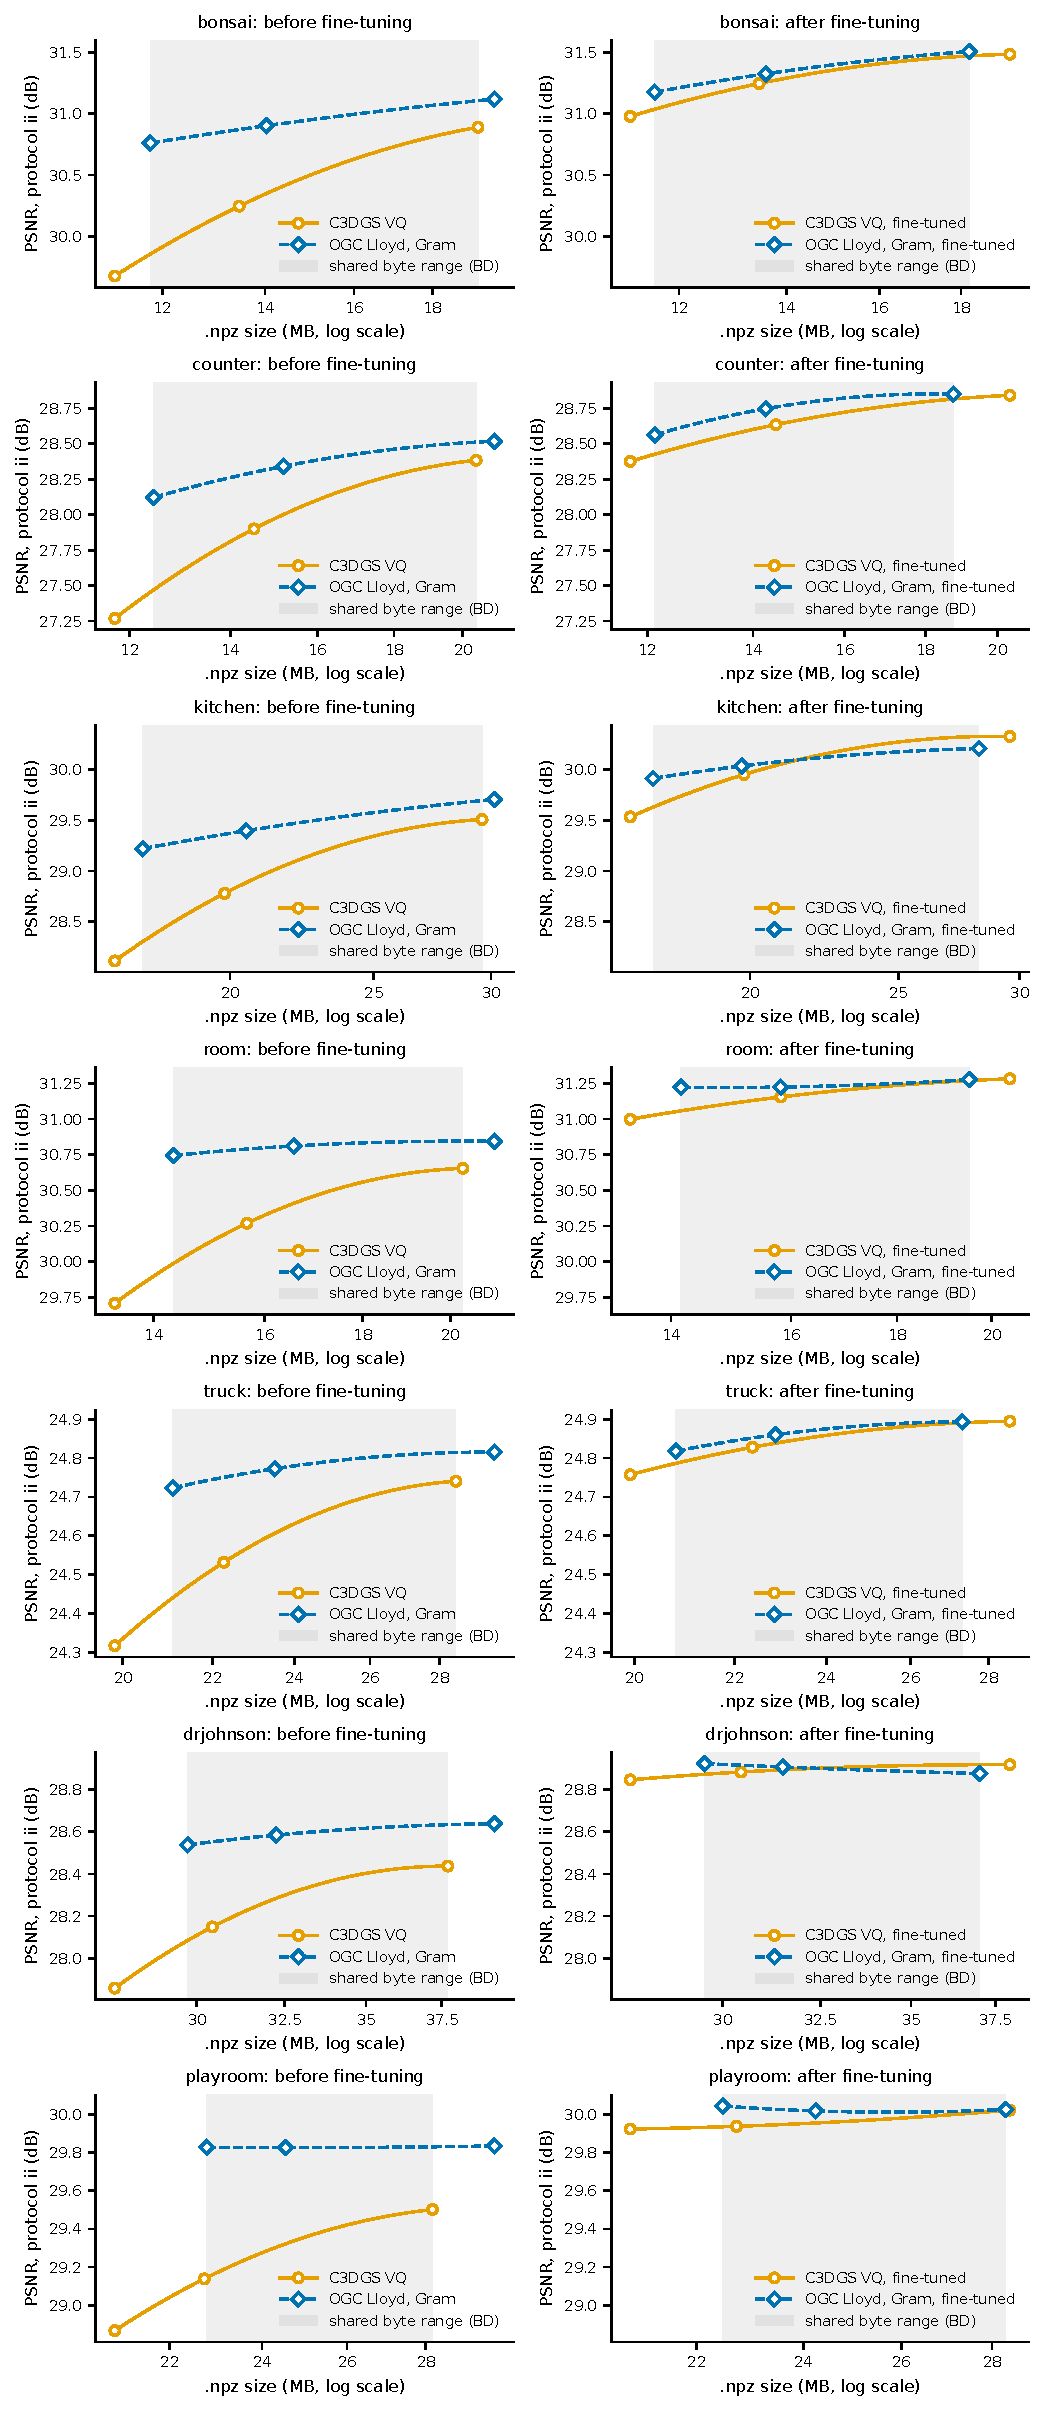
\includegraphics[width=\linewidth]{f1_rd_all.pdf}
\caption{Protocol~ii PSNR against \code{.npz} size (log scale) per gate scene, before (left) and after (right) C3DGS's fine-tuning, from E6 part (b): one process (seed 0) per point, each curve the parabola through its three points. The shaded band is the byte range the two curves share, over which BD-PSNR averages. The two panels of a scene share the PSNR axis.}
\label{fig:f1}
\end{figure}

\subsection{Caveats}

The test runs OGC's released VQ on this project's 16-probe estimate of OGC's metric, not on OGC's own Gram computation, so this replication (H1) replicates OGC's VQ given an estimated metric; a difference between our $G$ and OGC's own Gram, such as the trace shortfall on train (Section~\ref{sec:setup}), lies outside this test. % Am17 b; s16; E4
The result covers seven scenes, INRIA's published checkpoints, $K$~=~4,096 and three colour thresholds, on one host commit, one GPU type and one software image. % s19 "What E5 settles"; CLAIMS common E5 limits
Five of the seven scenes had been used earlier by this project with its own checkpoints, and four appear in OGC's paper (Section~\ref{sec:setup}). % Am15 d; CLAIMS common E5 limits
$\mathrm{SE}_{\mathrm{noise}}$ is seed noise at $j = 0$ only; it does not include how P varies from scene to scene, and the points at $j = -1$ and $j = +1$ have one seed each, so the noise of the BD values themselves was not measured. % s19 "What E5 settles"; A2; CLAIMS Gap 8
Each P rests on six measurements, since a parabola through three points per curve fits them exactly. % s19; A2
Before fine-tuning, the $j = 0$ difference of $+0.5239$ dB (95\% interval $+0.3798$ to $+0.6681$) sits beside OGC's reported $+0.49$ dB, but the two are not like for like: OGC's is a paired mean over nine Mip-NeRF 360 scenes, one run each, under its own evaluation and at a larger size than its reproduction, ours over seven scenes, four of them shared, under protocol~ii and at unequal bytes. % s19 secondaries; A4; RELATED_WORK_OGC.md section 2 g (OGC's Table 1)

% Section 4: the dissection. Sources: FINDINGS s16-s20, s24, s25; CLAIMS B1-B8, D5, D6, E13, E16-E18, F9, G7; Gaps conflicts 1-2.
% One sentence per line; each result sentence names its FINDINGS section (s##) and CLAIMS row in its trailing comment.
\section{Dissection}
\label{sec:dissection}

This section asks which parts of OGC's VQ carry its lead over C3DGS's own: the metric, the Lloyd algorithm around it, and how many codewords it uses. % Am17 b, d; s19, s20
Only Section~\ref{sec:gram-trace} is a pre-registered test; the rest is descriptive or exploratory, as labelled. % Am17 d; CLAIMS group B

\subsection{The Gram metric against its trace}
\label{sec:gram-trace}

P2, the BD-PSNR of \code{ogc\_gram} against \code{ogc\_scalar}, isolates the metric: both rows run OGC's own Lloyd, one with the per-splat $16\times16$ Gram matrix and one with its trace, $\operatorname{tr}(G_i)/16\cdot I$. % Am17 b, d
In OGC's own Lloyd the Gram metric beat its trace at equal rate on all seven gate scenes, with $\bar P_2 = 0.1874$ dB against $2\,\mathrm{SE}_{\mathrm{noise}} = 0.0003$ dB (pre-registered; E5's verdict, Section~\ref{sec:replication}). % s19 "The verdict"; B1
Per scene P2 ran from 0.1000 dB on truck to 0.3205 dB on bonsai (Table~\ref{tab:t1}). % s19 secondaries table; B1
$\mathrm{SE}_{\mathrm{noise}}$ is seed noise at $j = 0$ only; under $\mathrm{SD}_{\mathrm{pool}}/\sqrt{n}$, the standard error that matches one curve per scene, $\bar P_2$ lay 790.14 standard errors above zero, so criterion 3 held under either convention (analysis only). % s25; B1
As for P1, this is a replication on our estimate of OGC's metric (Section~\ref{sec:setup}). % Am17 b; A12

\subsection{From C3DGS's VQ to OGC's, step by step}
\label{sec:steps}

Between C3DGS's VQ and OGC's lie three steps, each a pair of rows in the same processes: OGC's Lloyd with the identity metric against C3DGS's VQ, the trace weight against the identity, and the Gram metric against its trace (P2). % Am17 b; s19
Both other steps were positive on every scene, in BD-PSNR and at $j = 0$: \code{ogc\_scalar} minus \code{ogc\_plain} had a paired mean of $+0.0613$ dB ($\mathrm{SE}_{\mathrm{noise}}$ 0.000125) and \code{ogc\_plain} minus \code{c3dgs} $+0.2167$ dB ($\mathrm{SE}_{\mathrm{noise}}$ 0.003220) (descriptive, pre-registered secondaries without bars). % s19 secondaries; B3
The mean BD-PSNR over the seven scenes was 0.1185 dB for the identity metric against C3DGS's VQ, 0.0520 dB for the trace weight against the identity, and 0.1874 dB for the Gram metric against its trace (exploratory, not pre-registered). % s19 "Exploratory"; B2
On the development scenes (E6 part (a), descriptive) the identity step, \code{ogc\_plain} against \code{c3dgs}, was negative on flowers ($-0.013664$ dB) and treehill ($-0.077859$ dB) and positive on train ($+0.057308$ dB), so its sign on the gate scenes does not carry over. % s23 "The predictions", d; G7
These are three separate BD values, each over its own pair's shared byte range, so they do not add: they sum to 0.3579 dB against P1's 0.3558 dB (Fig.~\ref{fig:f2}). % s19 "Exploratory"; B2
As a ratio of mean BD-PSNRs the Gram step is 52.7\% of P1. % s19 "Exploratory"; B2
That share must not be read as \emph{the} metric's share: on train, the development scene, the same step was 45.9\% of the $j = 0$ difference through OGC's Lloyd, and 65.4\% of a post-hoc chain through GN-VQ's code, and the three figures measure different paths on different scenes. % s17; s18; B4, B6; CLAIMS conflict 1

\begin{figure}[t]
\centering
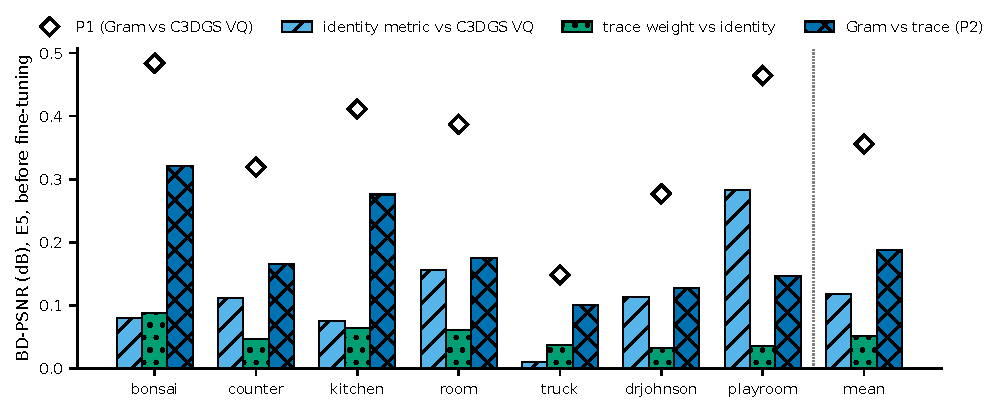
\includegraphics[width=\linewidth]{f2_p1_decomposition.pdf}
\caption{P1's steps per gate scene, E5 before fine-tuning (BD-PSNR over E5's seed-0 curves), stacked from the bottom: OGC's Lloyd with the identity metric against C3DGS's VQ, the trace weight against the identity, and the Gram metric against its trace (P2). The diamond is P1; on the mean it carries $\pm1$ standard error, $\mathrm{SD}_{\mathrm{pool}}/\sqrt{n}$, smaller than the marker. Each step is a BD value over its own pair's shared byte range, so the top of a stack is the steps' sum, not P1: over the seven scenes the steps' means sum to 0.3579 dB against P1's 0.3558 dB, and per scene the two differ by a few thousandths of a dB. Exploratory except P1 and P2.} % s19 "Exploratory"; s25; B2, A2
\label{fig:f2}
\end{figure}

\subsection{Codebook use}
\label{sec:codebook}

OGC's three rows used all 4,096 codewords in every process of every scene, while C3DGS's own VQ used 935 to 3,360, that is 22.8\% to 82.0\% of its codebook (pre-registered secondary, no bar; Fig.~\ref{fig:f5}). % s20 "Codewords used"; B8
Within a process every row shares the geometry, and only the colour arrays and the colour indices differ between rows. % s20 "Per-array bytes"; B8
Of OGC's extra bytes over C3DGS's at $j = 0$, 85.9\% to 95.0\% were its indices, which use the whole codebook nearly uniformly and so compress less. % s20 "Per-array bytes"; B8
BD-PSNR uses each row's whole \code{.npz} size, indices included. % s19 "How the numbers are computed"; A2

\begin{figure}[t]
\centering
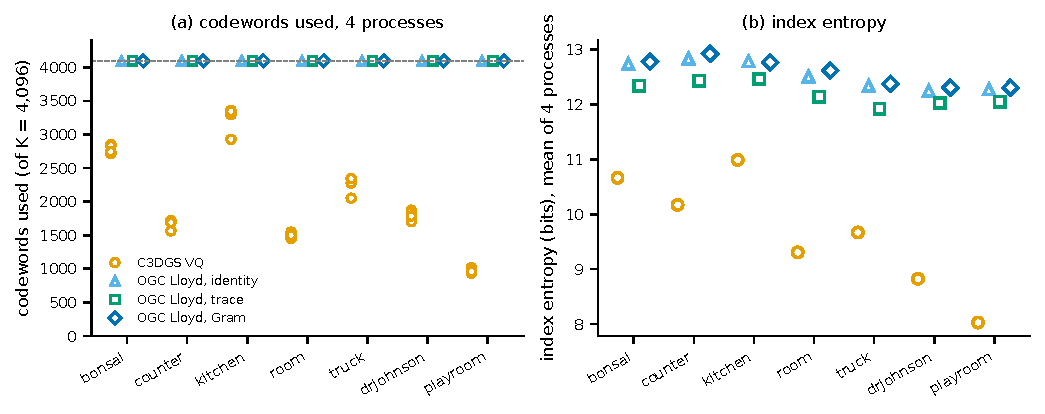
\includegraphics[width=\linewidth]{f5_codewords.pdf}
\caption{Codewords used (a) and index entropy (b) per method and gate scene, from E5's four processes per scene. OGC's three metrics use all 4,096 codewords in every process. Pre-registered secondaries, no bars.}
\label{fig:f5}
\end{figure}

\subsection{GN-VQ against OGC on the development scenes}
\label{sec:gnvq}

The project's own Gauss--Newton VQ (GN-VQ) was compared with OGC's VQ inside C3DGS only on the development scenes train and treehill, and never on a gate scene (exploratory, no verdict). % s17; Am16 b; D6
With all of OGC's algorithmic choices made in GN-VQ's code (\code{lad\_all}), GN-VQ came within 0.0013 dB of OGC's VQ on train and 0.0009 dB on treehill. % s17 "What E4q settles"; B5
The large single steps were the ones that fill empty codebook entries, reseeding ($+0.0394$ dB on train) and OGC's initial draw ($+0.0179$ dB on treehill), while each regularisation choice was worth 0.0097 dB or less, which is consistent with codebook use, rather than regularisation, being the gap between GN-VQ and OGC (exploratory, two development scenes). % s17 "What E4q settles"; B5
On train at equal rate OGC's VQ needed 14.42\% fewer bytes than GN-VQ (BD-PSNR $+0.0228$ dB), and GN-VQ's cross-validated floor was worth 0.0007 dB. % s17; s16; D6
On this evidence GN-VQ was retired from any gate before E5's code (Section~\ref{sec:setup}). % Am17 a; D6
These comparisons rest on two development scenes and do not bear on the gate scenes. % s17 "Not settled"; B5, D6

\subsection{The AC colour grid: bytes only}
\label{sec:ac-grid}

C3DGS stores the colour table through int8 quantisers whose grid, for every unfine-tuned row, is the checkpoint's own feature range, fitted to neither codebook (code reading). % s24 item 1; E16
Before fine-tuning OGC's AC codebook reached 159 to 389 grid steps beyond that grid, and 24 to 157 of its AC codebook values per process were clamped at the save, so P1 was measured with OGC's AC codebook clamped; C3DGS's AC codebook was never outside the grid (descriptive). % s24 item 2; E17
Fine-tuning re-fits the grid: OGC's AC scale grew by a factor of 1.59 to 3.16 and its \code{.npz} shrank by 10.68\% to 0.63\%, while C3DGS's AC scale changed by a factor of 0.80 to 1.13 and its \code{.npz} by $-0.31\%$ to $+1.01\%$ (descriptive; Fig.~\ref{fig:f4}). % s22 e; F9
What this records is the re-fit's effect on bytes. % s24; F9, E13
Its effect on the PSNR lead is untested, and the exploratory correlations run the wrong way for it to be the cause: across the seven scenes a larger widening of OGC's AC grid went with a smaller, not larger, fine-tuning gain difference (exploratory, $n = 7$; Spearman $\rho = -0.89$, $-0.21$ over the 28 processes and $-0.30$ after the gap-closing trend is removed). % s24 item 6; E18
E7 holds the grids, the codewords and the rest of fine-tuning fixed in turn to test this (Section~\ref{sec:ft-why}). % Am20 a; CLAIMS Gap 3

\begin{figure}[t]
\centering
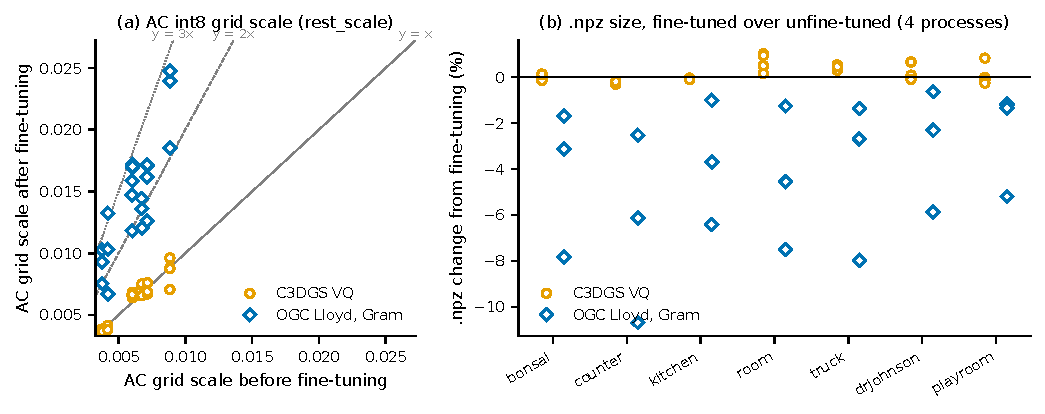
\includegraphics[width=\linewidth]{f4_ac_refit.pdf}
\caption{Fine-tuning re-fits the AC colour grid (E6 part (b), the seven gate scenes; descriptive). AC: the SH coefficients of degrees 1--3 (\code{features\_rest}). One point is one process of one scene (four per scene: $j = -1, 0, +1$ with seed 0 and $j = 0$ with seed 1), for C3DGS's VQ and for OGC's Gram-metric VQ. (a) The AC int8 grid's scale (\code{rest\_scale} of the quantizer at the save) after fine-tuning against before, with the lines $y = x$, $2x$ and $3x$. (b) The \code{.npz} size change from fine-tuning, per scene.} % s22 e; F9
\label{fig:f4}
\end{figure}

% Section 5: fine-tuning. 5.1 written (E6, H2); 5.2 a stub until E7's verdict. Sources: FINDINGS s19-s23, s25;
% CLAIMS A5, F1-F8, G1-G7, conflict 3. One sentence per line; each result sentence names its s## and CLAIMS row.
\section{Fine-tuning}
\label{sec:finetuning}

\subsection{The lead after fine-tuning}
\label{sec:ft-result}

\paragraph{Hypothesis and test.}
E6 part (b) asked whether OGC's Gram-metric VQ still beats C3DGS's own colour VQ at equal rate after C3DGS's 5,000-iteration fine-tuning, on the seven gate scenes (P\_FT, BD-PSNR of \code{ogc\_gram\_ft} against \code{c3dgs\_ft}, computed as P1 with the fine-tuned rows). % Am19 c; s21
It used E5's three criteria on fresh processes, four per scene, each fine-tuning both rows, so that the fine-tuned rows have a curve over the three colour thresholds. % Am19 c; s21
The hypothesis was formed after seeing E5's results on these scenes, so this is a pre-registered test on them and not a held-out claim. % Am19 c; s21; CLAIMS group F limits

\paragraph{Result (pre-registered).}
E6 part (b) passed as pre-registered: after fine-tuning OGC's VQ led C3DGS's own at equal rate with $\bar P_{\mathrm{FT}} = 0.0425$ dB, positive on 6 of 7 scenes, and $\bar P_{\mathrm{FT}} = 4.9\,\mathrm{SE}_{\mathrm{noise}}$ against the required 2 ($2\,\mathrm{SE}_{\mathrm{noise}} = 0.0174$ dB). % s21 "The verdict"; F1
The one negative scene was drjohnson, at $-0.0046$ dB (Table~\ref{tab:t2a}). % s21 per-scene table; F1
No scene was dropped and no primary row or value was missing. % s21 "The verdict"; F1

\begin{table}[t]
\centering
\footnotesize
\setlength{\tabcolsep}{4pt}
\caption{E6 part (b) per scene (dB). P\_FT is the pre-registered primary (9 decimals, as compared). $D_{s0}$ and $D_{s1}$ are the fine-tuned pair's protocol~ii difference at $j = 0$ with seeds 0 and 1, $D_s$ their mean and $v_s$ their sum of squared deviations. P1 replicated is a report-only secondary beside E5's P1. Generated from the committed bundles.}
\label{tab:t2a}
% FINDINGS section 21 (verdict table, secondary 1); E6 part (b), kaggle/gn_e6/S1-S3/gn6/
% generated by paper/figs/t2_e6_pft.py from committed bundles; do not edit
\begin{tabular}{lrrrrrrr}
\toprule
Scene & P\_FT (dB) & $D_{s0}$ & $D_{s1}$ & $D_s$ & $v_s$ & P1 repl. & P1 E5 \\
\midrule
bonsai & 0.062187712 & +0.079084 & +0.091531 & +0.085308 & 7.75e-05 & 0.4817 & 0.4841 \\
counter & 0.105805442 & +0.112069 & +0.036106 & +0.074087 & 2.89e-03 & 0.3197 & 0.3192 \\
kitchen & 0.012493186 & +0.083968 & +0.021124 & +0.052546 & 1.97e-03 & 0.4073 & 0.4111 \\
room & 0.056026648 & +0.069505 & +0.008662 & +0.039084 & 1.85e-03 & 0.3914 & 0.3869 \\
truck & 0.017281080 & +0.032199 & +0.031499 & +0.031849 & 2.45e-07 & 0.1484 & 0.1486 \\
drjohnson & -0.004616264 & +0.023915 & -0.011068 & +0.006424 & 6.12e-04 & 0.2757 & 0.2765 \\
playroom & 0.048257314 & +0.080564 & +0.074441 & +0.077502 & 1.87e-05 & 0.4651 & 0.4644 \\
\midrule
$\bar P$ ($n = 7$) & 0.042490731 &  &  &  &  & 0.3556 &  \\
SD\_pool & 0.032555899 &  &  &  &  &  &  \\
SE\_noise = SD\_pool / $\sqrt{14}$ & 0.008700930 &  &  &  &  & 0.0030 &  \\
2 $\times$ SE\_noise & 0.017401860 &  &  &  &  &  &  \\
scenes with P > 0 & 6 (5 needed) &  &  &  &  & 7 of 7 &  \\
\bottomrule
\end{tabular}

\end{table}

\begin{table}[t]
\centering
\small
\caption{E6 part (b), leave-one-out (descriptive, not pre-registered): the three criteria over the six scenes left when the row's scene is removed. Generated from the committed bundles.}
\label{tab:t2b}
% FINDINGS section 22 a (leave-one-out, descriptive); E6 part (b), kaggle/gn_e6/S1-S3/gn6/
% generated by paper/figs/t2_e6_pft.py from committed bundles; do not edit
\begin{tabular}{lrrrll}
\toprule
Left out & $\bar P$ & SE\_noise & $\bar P$ / SE\_noise & Positive & Criteria 1 / 2 / 3 \\
\midrule
bonsai & 0.039208 & 0.010098 & 3.88 & 5 of 6 (5 needed) & yes / yes / yes \\
counter & 0.031938 & 0.007936 & 4.02 & 5 of 6 (5 needed) & yes / yes / yes \\
kitchen & 0.047490 & 0.008696 & 5.46 & 5 of 6 (5 needed) & yes / yes / yes \\
room & 0.040235 & 0.008794 & 4.58 & 5 of 6 (5 needed) & yes / yes / yes \\
truck & 0.046692 & 0.010151 & 4.60 & 5 of 6 (5 needed) & yes / yes / yes \\
drjohnson & 0.050342 & 0.009723 & 5.18 & 6 of 6 (5 needed) & yes / yes / yes \\
playroom & 0.041530 & 0.010138 & 4.10 & 5 of 6 (5 needed) & yes / yes / yes \\
\bottomrule
\end{tabular}

\end{table}

\paragraph{How firm the result is (descriptive, not pre-registered).}
Leaving out any one scene (Table~\ref{tab:t2b}), every case still met all three criteria, with $\bar P / \mathrm{SE}_{\mathrm{noise}}$ from 3.88 to 5.46, but 6 of the 7 cases met the count with exactly 5 positive scenes, so the count is the tight criterion. % s22 a; F5
Across scenes P\_FT had a standard deviation of 0.0373 dB ($t = 3.0$), which $\mathrm{SE}_{\mathrm{noise}}$ does not measure. % s22 a; F5
Under the standard error that matches one curve per scene, $\mathrm{SD}_{\mathrm{pool}}/\sqrt{n}$, $\bar P_{\mathrm{FT}}$ lay 3.45 standard errors above zero against the registered 4.9, and the leave-one-out cases 2.75 to 3.86; criterion 3 still held in every case, and the registered verdict stands under its pre-registered rule. % s25; F1, F5
With OGC's bytes set to C3DGS's at each $j$, a counterfactual and not equal rate, the mean was $+0.0458$ dB against $\bar P_{\mathrm{FT}} = +0.0425$ dB, so the result is not produced by where the bytes fall. % s22 c; F7

\paragraph{Against the lead before fine-tuning (descriptive).}
As a ratio of means P\_FT was 0.1195 of P1 replicated, with per-scene ratios from $-0.017$ to $+0.331$; the two measures average over different byte ranges, so the ratio is not the share of the earlier lead that survives at any one rate. % s22 b; F6
E5's own $j = 0$ comparison after fine-tuning, $+0.0604$ dB at unequal bytes, measures a different quantity on separate runs; neither value replaces the other. % s19 secondaries; A5; CLAIMS conflict 3

\paragraph{Where along the curve (descriptive, not pre-registered).}
On all seven gate scenes the fine-tuned rows' PSNR difference at the same $j$ rose from $j = -1$ to $j = +1$: from $-0.119$ to $+0.023$ dB at $j = -1$, $+0.024$ to $+0.112$ dB at $j = 0$, and $+0.061$ to $+0.379$ dB at $j = +1$. % s22 d; F8
These points are not rate-matched: at $j = +1$ OGC's row had 3.5\% to 7.9\% more bytes, and at $j = -1$ 0.3\% to 7.9\% fewer. % s22 d; s21 secondary 2; F8
After fine-tuning OGC's \code{.npz} was smaller than C3DGS's at $j = -1$ on every scene and larger at $j = +1$ on every scene, while before fine-tuning it was larger at every point. % s21 secondary 2; F3
The rising pattern is scoped to the gate scenes: on the development scenes it rose on flowers but fell on train and was not monotone on treehill. % s23 e; F8, G5

\paragraph{The development scenes (descriptive).}
E6 part (a) ran the same rows on flowers, treehill and train with three predictions and no criterion (Table~\ref{tab:t3}). % Am19 b; s23; CLAIMS group G limits
All three predictions held on all three scenes: P1 $> 0$, P2 $> 0$, and P\_FT below P1. % s23 "The predictions"; G1
P\_FT was $+0.0341$ dB on flowers and negative on treehill ($-0.0262$ dB) and train ($-0.0066$ dB), so the third prediction held on treehill and train because P\_FT was negative. % s23 "The predictions"; G1, G2
Treehill's P\_FT stayed negative with the $j = 0$ seed-1 process in place of seed 0 ($-0.0423$ dB). % s23 b; G2
Train's P\_FT is not interpreted: its fine-tuned points moved by up to 0.19 dB between runs, and replacing its $j = 0$ fine-tuned point with the pilot's changed it by $+0.2274$ dB. % s23 a; G3
These are development scenes; no part (a) value is pooled with the gate scenes' results. % Am19 b; CLAIMS group G limits

\begin{table}[t]
\centering
\small
\caption{E6 part (a) on the development scenes (BD-PSNR, dB). Descriptive: three predictions checked, no criterion. Generated from the committed bundles.}
\label{tab:t3}
% FINDINGS section 23, The predictions (E6 part (a), descriptive; kaggle/gn_e6/S4-S5/gn6/)
% generated by paper/figs/t3_e6_part_a.py from committed bundles; do not edit
\begin{tabular}{lrrrrrl}
\toprule
Scene & P1 & P2 & scalar vs plain & plain vs c3dgs & P\_FT & Predictions 1 / 2 / 3 \\
\midrule
flowers & +0.123913 & +0.069250 & +0.068761 & -0.013664 & +0.034106 & held / held / held \\
treehill & +0.025062 & +0.002488 & +0.102726 & -0.077859 & -0.026188 & held / held / held \\
train & +0.129723 & +0.064938 & +0.008808 & +0.057308 & -0.006562 & held / held / held \\
\bottomrule
\end{tabular}

\end{table}

\paragraph{The curves.}
The right panels of Figure~\ref{fig:f1} show the fine-tuned curves; each scene's two panels share the PSNR axis, and the shaded band marks the byte range over which P\_FT averages. % paper/figs/f1_rd_curves.py; s21

\subsection{Why the lead shrinks (E7, pending)}
\label{sec:ft-why}

\TODO{E7 (Amendment 20): the within-process dissection of the shrink (arms R, G, CG, K, O). Written after all eleven sessions and E7's verdict; no mechanism is stated before then.}

% Section 6: stub (audit outline item 6). Sources when written: the CLAIMS limit columns, Gaps 3, 4, 7, 8, 12, 13.
\section{Limits}
\label{sec:limits}

\TODO{Limits: scenes and checkpoints, one host and one GPU type, three points per curve and BD-level noise, the SE convention, protocol ii against C3DGS's evaluation, the comparison with OGC's paper that is not like for like.}


\appendix
% Appendix: stub (audit outline item 7).
\section{Appendix}
\label{sec:appendix}

\TODO{Appendix: the full amendment history, the session records, per-scene F1 panels, the checkers and how to rerun them.}


\bibliographystyle{plainnat}
\bibliography{references}

\end{document}
